\documentclass[12pt]{article}
\usepackage{amsmath}
\usepackage{mathtools}
\usepackage{bigints}
\usepackage{parskip}
\usepackage{amssymb}
\usepackage{relsize}
\usepackage{fullpage}
% \DeclareMathSizes{12}{17.28}{9}{7} % (a)

\DeclareMathSizes{12}{17.28}{12}{12} % (a)


\usepackage{hyperref}



	\addtolength{\topmargin}{-.5in}
	\addtolength{\textheight}{1.75in}



    \newenvironment{myindentpar}[1]%
     {\begin{list}{}%
             {\setlength{\leftmargin}{#1}}%
             \item[]%
     }
     {\end{list}}

\begin{document}
\title{College Algebra: Module 14 What You Need To Know}
\date{3-28-15}
\author{}
\maketitle

\section{Linear Systems in Two Variables with Applications (Section 6.1)}

When solving linear systems of equations in \textit{two or three variables} there will always be \textbf{one of three possible solutions}:

\begin{enumerate}

\item \textbf{One Solution} (Consistent Independent System)
\item \textbf{No Solution} (Inconsistent System)
\item \textbf{Infinitely Many Solutions} (Consistent Dependent System)

\end{enumerate}

\vspace{1cm}

We will learn three methods for solving systems of equations in \textit{two} variables:


\begin{enumerate}
\item \textbf{Graphical Method}
\item \textbf{Substitution Method}
\item \textbf{Elimination Method}
\end{enumerate}

\vspace{.5cm}

\textbf{Graphical Method:}

- This involves graphing the two lines you're given and finding the point of intersection between the two lines. If there is only one point of intersection, then the solution will be that point. If the lines are parallel then there will be no solution and if the lines are the same, there will be infinitely many solutions. See the picture below for a graphical representation of what this means:

\centerline{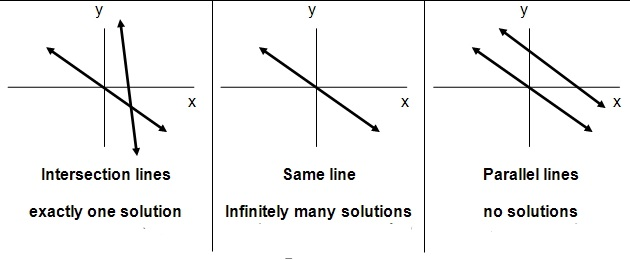
\includegraphics{LinearSystemSoln.jpg}}

See the examples on the following pages for the difference between the \textbf{Substitution Method} and \textbf{Elimination Method}:

\textbf{Substitution Method:}

\centerline{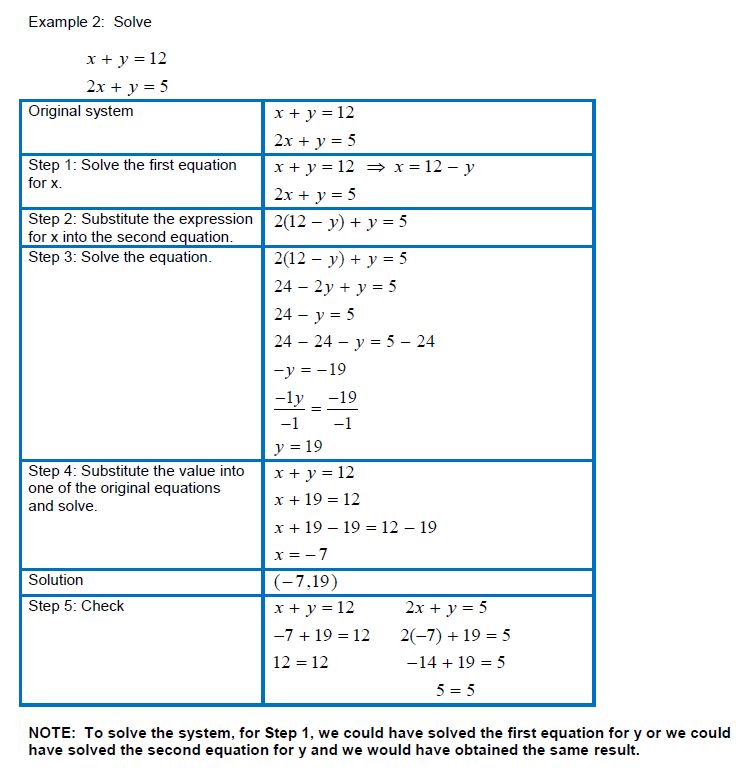
\includegraphics[scale = 0.9]{Substitution.png}}

\newpage

\textbf{Elimination Method:}

\centerline{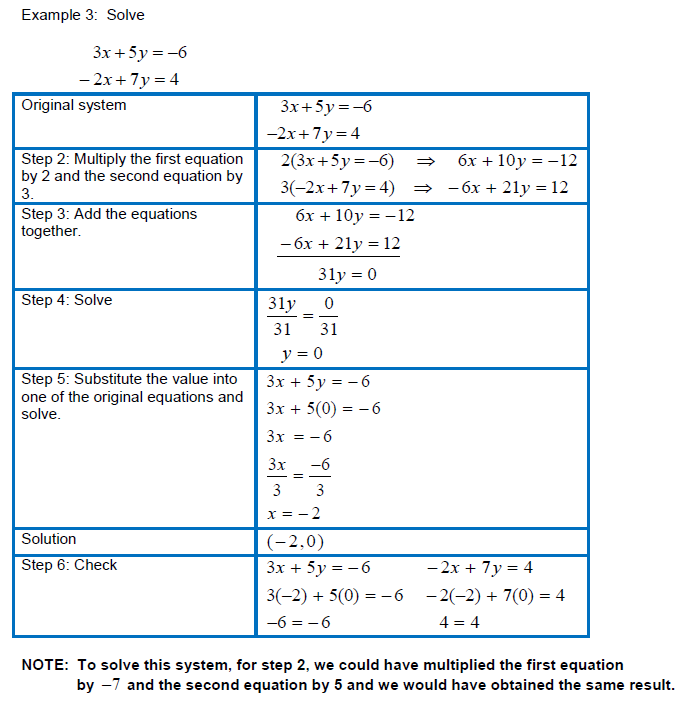
\includegraphics{Elimination.png}}

\section{Linear Systems in Three Variables with Applications (Section 6.2)}

- Just going to do example problems in class. There are no formulas you need to know for this. You just need to see example problems of how to solve these. The general idea is to use the \textbf{Elimination Method} that we saw for solving linear systems of equations with two variables. Except, the only difference now is that instead of solving for \textbf{two variables} $x$ and $y$, now we are solving for \textbf{three variables}: $x$, $y$, and $z$



















\end{document}